\documentclass[10pt, a4paper]{article}

\usepackage{parskip} 				

\begin{document}
\begin{center}
\Huge{Part II Project - Plan for Evaluation} \par
\Large{March 2023} \par
\end{center}
\par
\par

\section*{Overview}
The evaluation for the mobile ad-hoc network (MANET) will be split into two parts -- first the evaluation for the pure MANET and a whole system evaluation. The evaluation of the MANET will examine the implementation of Epidemic, the delay tolerant networking protocol will be checked for correctness and performance. The system evaluation will look at the MANET in the context of the use case, on the water.  \\ \\
All data will be logged on the node in a CSV file with columns \\ \verb'Node Address, Time, Time Since Node Startup, Event Type, Event Information' \\ where the Event Information varies with the event being logged and may contain the GPS location and message keys. This data will then be analysed on my device using Python code.

\section*{Evaluating the MANET}
These tests be conducted in a field, as this will give an outdoor environment similar to the use case, but I will be able to better control the conditions the node is in. They will use four nodes, as this is the maximum number of nodes we can accurately calculate time for. Two nodes will use GPS to find the current time and two will use the serial connection to laptops to calculate the time. These tests will be conducted first on a small scale, with short tests using a small number of nodes, to ensure the tests can be run. After this has been confirmed, the tests will be run for a longer time with the maximum number of nodes. \\  \\
The tests can then be compared to the evaluation in the initial epidemic paper \hyperref[epidemic]{[3]}, which simulated the nodes with 50 mobile nodes in a 1500 x 300 m space using the Monarch extensions to the ns-2 packet-level simulator rather than hardware as I am doing. Evaluation metrics examined included message delivery latency, delivery rate, the average and maximum number of hops a message took to get to a node.\\ \\
The first test will be the percentage of packets delivered in the four node network. This will be time limited (i.e. if a message is not received in x minutes, it is considered undelivered). Nodes will randomly generate a new message every second, for a total of 25 messages, mirroring the structure of testing used in Vahdat and Becker's paper \hyperref[epidemic]{[3]}. The nodes will be in a box of area $20m^2$ with the range of the radios reduced to approximately $5m$ to simulate the environment in which the system will be used. The nodes will move constantly. \\  \\ 
Next, the transfer delay will be measured. This will be the average time taken for each message to be delivered, and will use the same setup as percentage of packets delivered testing. \\ \\
\begin{figure}[h]
\caption{The setup and axes for delivery rate and transfer delay}
\begin{center}
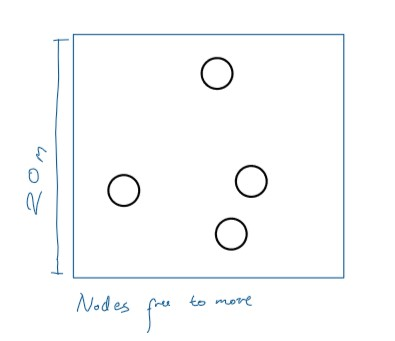
\includegraphics[scale=0.5]{transfer.jpg}
\end{center}
\end{figure}
Finally, the time taken to propagate messages after partition will be measured. This will include one-sided, asymmetric partitions, where only one set of nodes has messages the other set has not seen. It will also include symmetric partitions, where both sets of nodes have messages the other set has not seen. The number of unseen messages will be increased and each test will be run five times.

\begin{figure}[h]
\caption{The setup and axes for partition testing}
\begin{center}
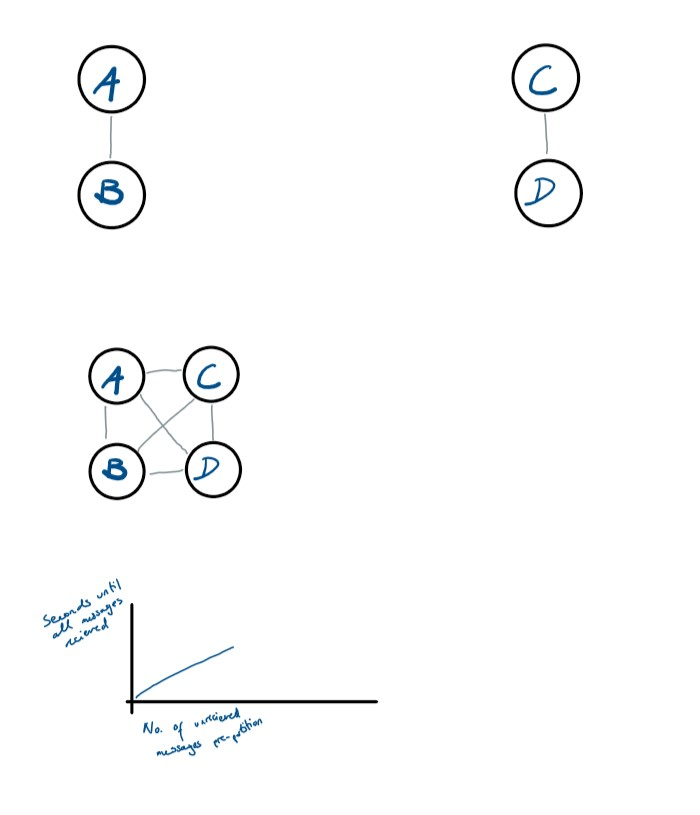
\includegraphics[scale=0.3]{partition.jpg}
\end{center}
\end{figure}


%sketch out graphs you will use
%Add pictures of the node teting setup 
%What will be evaluated and how?
%How to evaluate correctness? 
%How to do sensitivity on the data / metrics - how certain are we that this works..? 

\FloatBarrier
\section*{Evaluating the System}
This will be performed on the water, the environment the MANET will be used in, after a `dry run' on land to ensure there are no obvious flaws with the system. 
To examine the use of the system and how long it takes messages to arrive at other nodes, a well known obstacle has been selected. This is the red buoy at 51.48236626931181, -0.22641424521527762, shown below \hyperref[maps]{[1]}. Using the time given from the GPS chips, we can then map the locations and time since the obstacle was added that other nodes receive messages about the buoy. This experiment will be run multiple times to gather a sufficient volume of data about the propagation of new obstacles. \\ \\ 
Additionally, this will allow me to look at the behaviour of users when adding a new obstacle then tweak the MANET to fit. While there is a ground truth about the location of an obstacle, it is likely that most users will not be directly above the obstacle when they log it. 

\begin{figure}[h]
\caption{The location of the `red buoy' obstacle \hyperref[maps]{[1]}}
\begin{center}
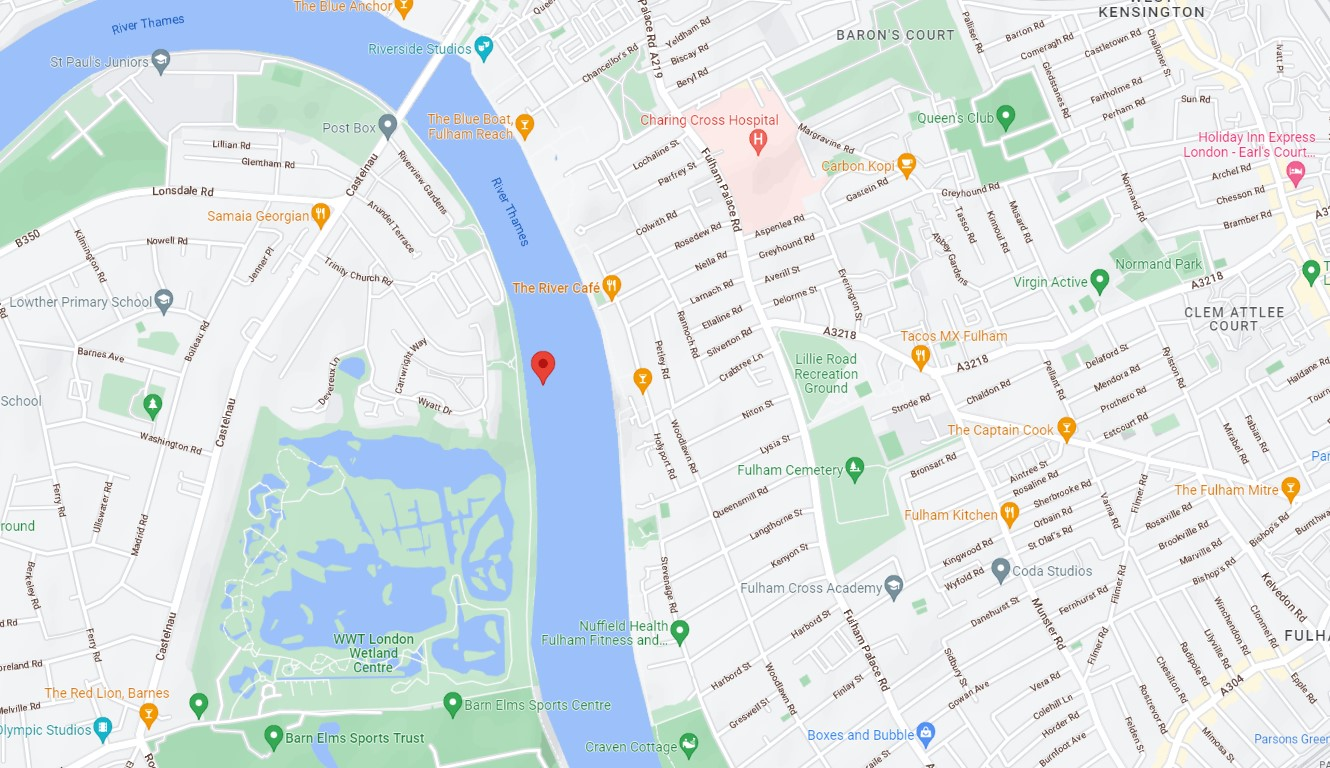
\includegraphics[scale=0.3]{buoy.jpg}
\end{center}
\end{figure}

\begin{figure}[h]
\caption{An image of the `red buoy' obstacle}
\begin{center}
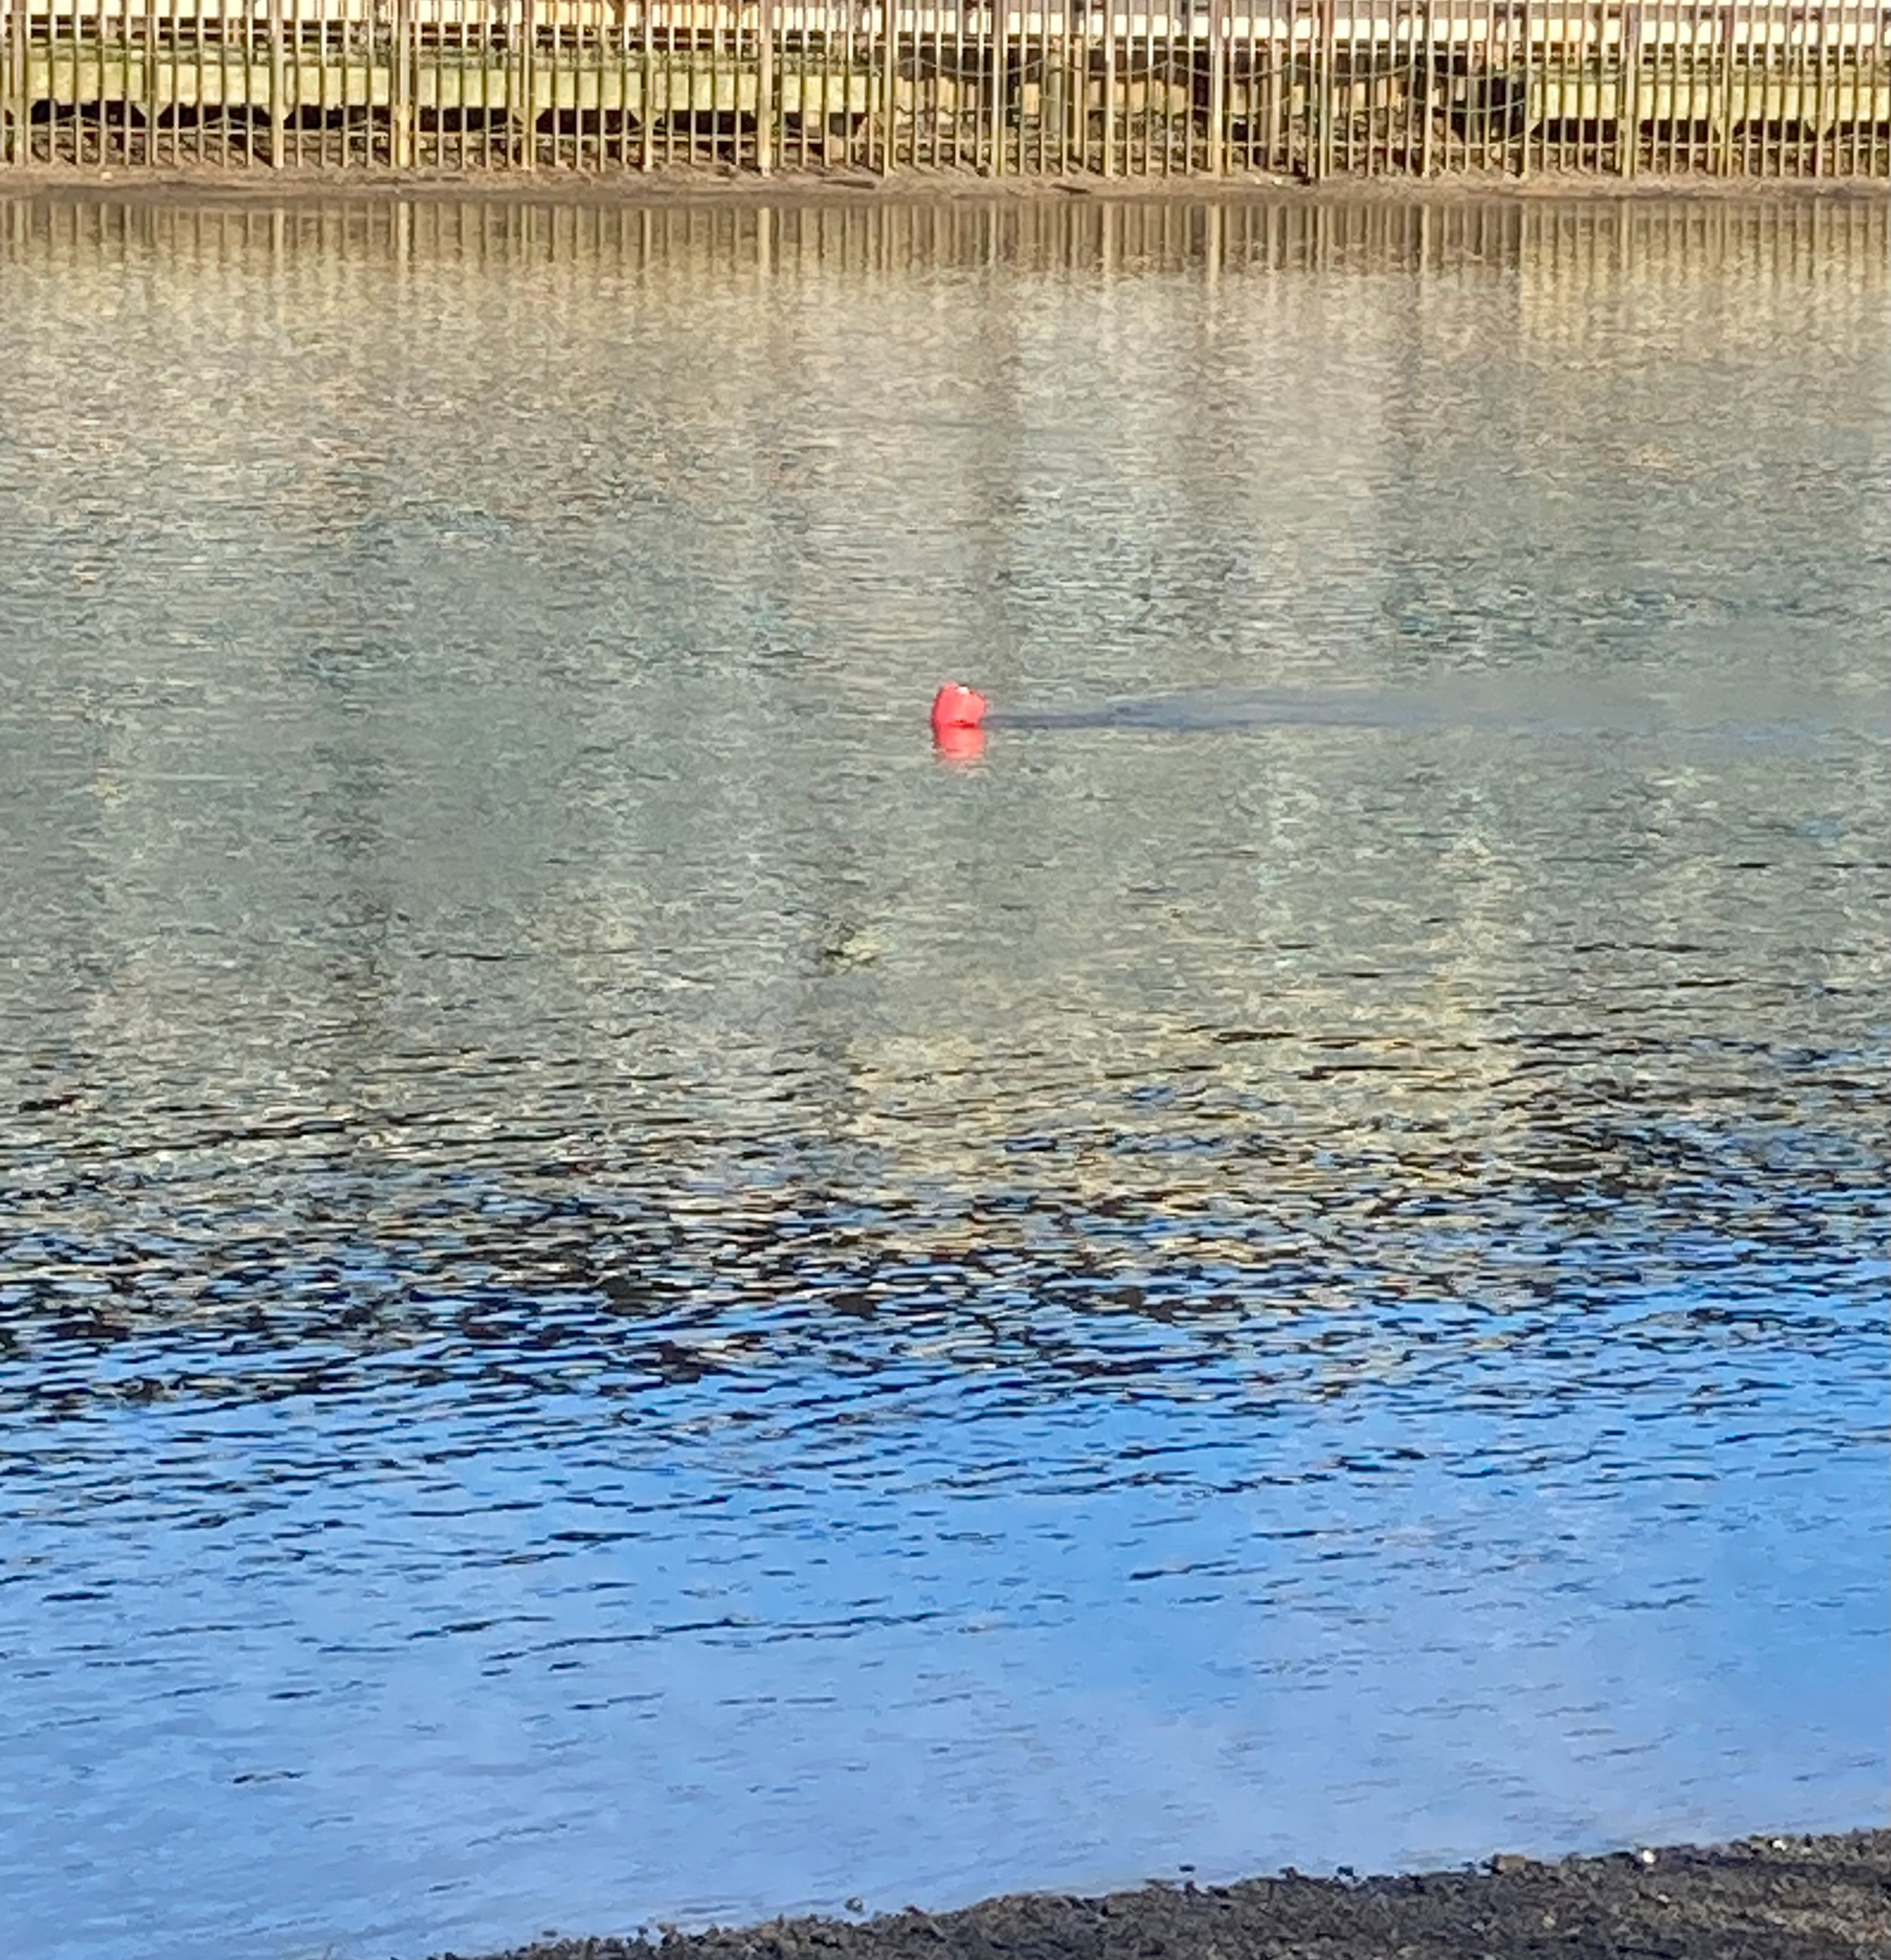
\includegraphics[scale=0.1]{buoy2.jpg}
\end{center}
\end{figure}
\FloatBarrier

\section*{Extensions}
If there is sufficient time, further evaluation can be performed on the MANET. This will be structured in a similar way to the tests in the `Evaluating the MANET'. Bandwidth will be tested in a fully connected network, where the number of messages per second transferred between two nodes may be found by generating random packets at set intervals at one node (node A shown below), and seeing how many are passed to another node (node B below). 
This test could then be performed with both nodes generating and receiving messages, to examine bandwidth on a two way connection.\\
\begin{figure}[h]
\caption{The setup and expected graph for testing bandwidth}
\begin{center}
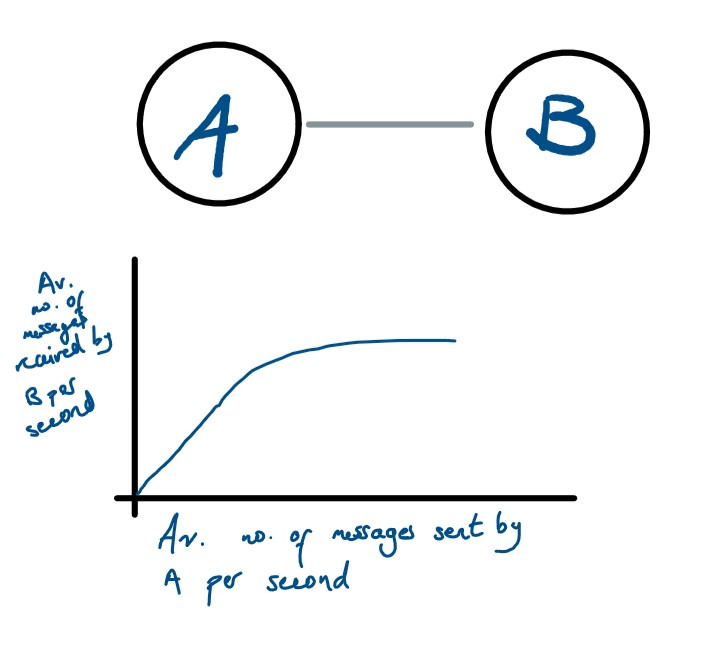
\includegraphics[scale=0.3]{bandwidth.jpg}
\end{center}
\end{figure}
Further extensions to the system evaluation will include a questionnaire for those who use the device, covering a range of users, including both coxes in coxed boats and rowers in coxless boats. \\ 

\FloatBarrier
\vspace{10px}
\section*{References}
\label{maps}[1] Google Maps. 51.4823, -0.2264. [Online] Available at: \url{https://www.google.co.uk/maps/place/51%C2%B028'56.5%22N+0%C2%B013'35.1%22W/@51.4820341,-0.2295313,15.5z/data=!4m4!3m3!8m2!3d51.4823663!4d-0.2264142!5m1!1e4} [Accessed March 2023] \\ \\
\label{epidemic}[3] Vahdat, A, Becker, D. Epidemic Routing for Partially-Connected Ad Hoc Networks. Published 2000. Duke University.
\end{document}






